\documentclass[tikz,border=8pt]{standalone}
% Shared look for every TikZ diagram. Load with % Shared look for every TikZ diagram. Load with % Shared look for every TikZ diagram. Load with \input{../../tools/tikz-style.tex}
\usepackage[T1]{fontenc}
\usepackage{lmodern}
\renewcommand{\sfdefault}{lmr}  % diagrams use the same serif as the text
\usetikzlibrary{arrows.meta, positioning, shapes.geometric, calc, fit, backgrounds}
\definecolor{cblue}{HTML}{4C78A8}
\definecolor{corange}{HTML}{F58518}
\definecolor{cgreen}{HTML}{54A24B}
\definecolor{cred}{HTML}{E45756}
\definecolor{cpurple}{HTML}{B279A2}
\definecolor{cgrey}{HTML}{6B6B6B}
\tikzset{
  every picture/.style={font=\sffamily, line width=1.2pt},
  box/.style={draw=#1, fill=#1!12, rounded corners=4pt, align=center, inner sep=7pt, minimum height=1.1cm},
  box/.default=cgrey,
  arrow/.style={-{Stealth[length=3mm]}, draw=cgrey, line width=1.4pt},
  title/.style={font=\sffamily\bfseries\Large},
  note/.style={font=\sffamily\small, text=cgrey, align=center},
}
\AtBeginDocument{\hyphenpenalty=10000 \exhyphenpenalty=10000}

\usepackage[T1]{fontenc}
\usepackage{lmodern}
\renewcommand{\sfdefault}{lmr}  % diagrams use the same serif as the text
\usetikzlibrary{arrows.meta, positioning, shapes.geometric, calc, fit, backgrounds}
\definecolor{cblue}{HTML}{4C78A8}
\definecolor{corange}{HTML}{F58518}
\definecolor{cgreen}{HTML}{54A24B}
\definecolor{cred}{HTML}{E45756}
\definecolor{cpurple}{HTML}{B279A2}
\definecolor{cgrey}{HTML}{6B6B6B}
\tikzset{
  every picture/.style={font=\sffamily, line width=1.2pt},
  box/.style={draw=#1, fill=#1!12, rounded corners=4pt, align=center, inner sep=7pt, minimum height=1.1cm},
  box/.default=cgrey,
  arrow/.style={-{Stealth[length=3mm]}, draw=cgrey, line width=1.4pt},
  title/.style={font=\sffamily\bfseries\Large},
  note/.style={font=\sffamily\small, text=cgrey, align=center},
}
\AtBeginDocument{\hyphenpenalty=10000 \exhyphenpenalty=10000}

\usepackage[T1]{fontenc}
\usepackage{lmodern}
\renewcommand{\sfdefault}{lmr}  % diagrams use the same serif as the text
\usetikzlibrary{arrows.meta, positioning, shapes.geometric, calc, fit, backgrounds}
\definecolor{cblue}{HTML}{4C78A8}
\definecolor{corange}{HTML}{F58518}
\definecolor{cgreen}{HTML}{54A24B}
\definecolor{cred}{HTML}{E45756}
\definecolor{cpurple}{HTML}{B279A2}
\definecolor{cgrey}{HTML}{6B6B6B}
\tikzset{
  every picture/.style={font=\sffamily, line width=1.2pt},
  box/.style={draw=#1, fill=#1!12, rounded corners=4pt, align=center, inner sep=7pt, minimum height=1.1cm},
  box/.default=cgrey,
  arrow/.style={-{Stealth[length=3mm]}, draw=cgrey, line width=1.4pt},
  title/.style={font=\sffamily\bfseries\Large},
  note/.style={font=\sffamily\small, text=cgrey, align=center},
}
\AtBeginDocument{\hyphenpenalty=10000 \exhyphenpenalty=10000}

\begin{document}
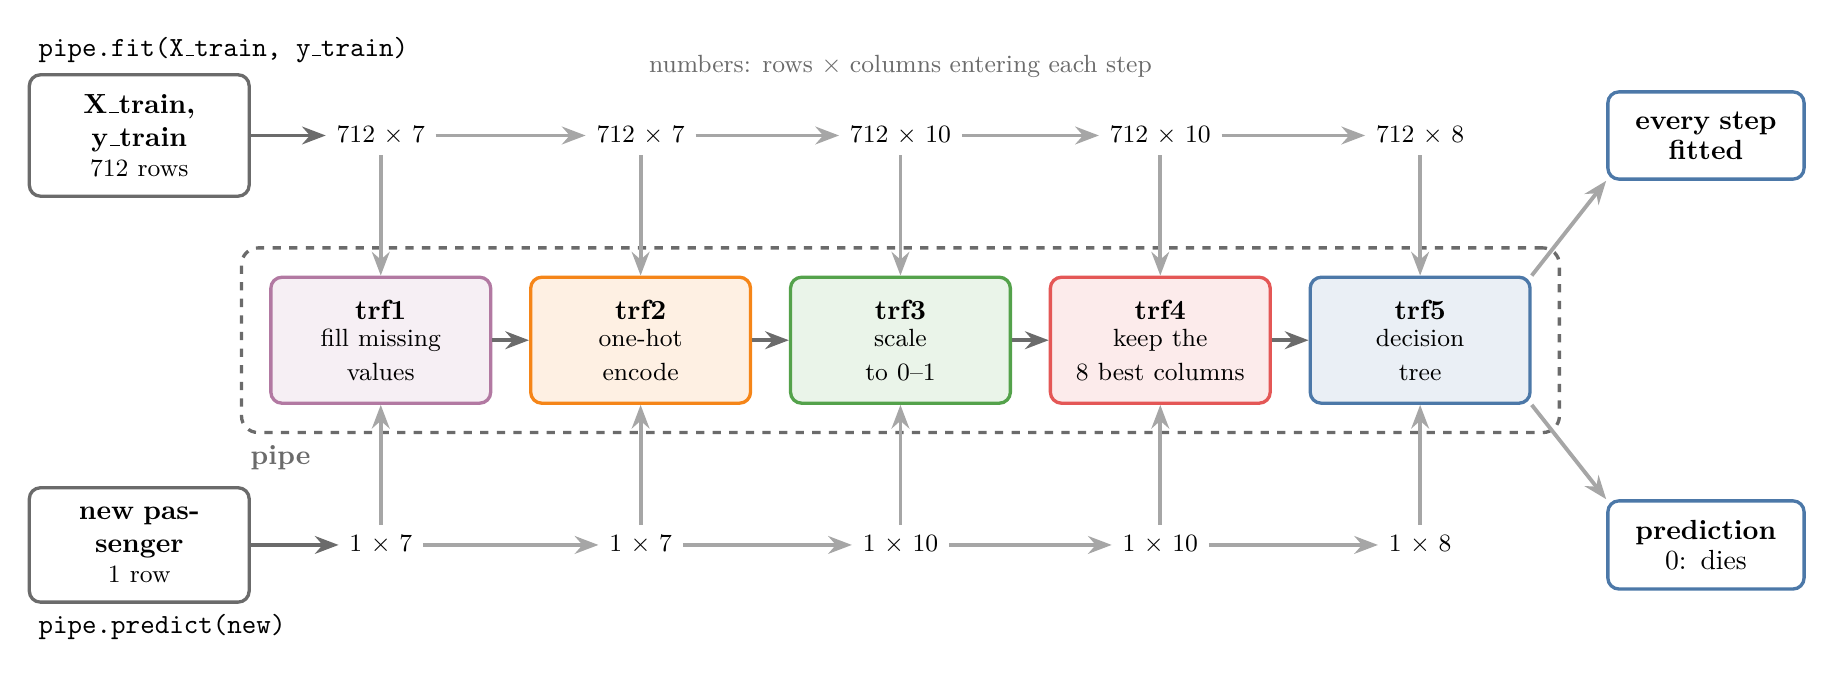
\begin{tikzpicture}
  % the five steps of one pipeline object
  \foreach \i/\c/\n/\job in {
      1/cpurple/trf1/fill missing\\values,
      2/corange/trf2/one-hot\\encode,
      3/cgreen/trf3/scale\\to 0--1,
      4/cred/trf4/keep the\\8 best columns,
      5/cblue/trf5/decision\\tree} {
    \node[box=\c, text width=2.3cm, minimum height=1.6cm] (s\i) at (3.3*\i,0) {\textbf{\n}\\[-1pt]\small \job};
  }
  \foreach \i [evaluate=\i as \j using int(\i+1)] in {1,2,3,4} { \draw[arrow] (s\i) -- (s\j); }
  \node[draw=cgrey, dashed, rounded corners=6pt, inner sep=10pt, fit=(s1)(s5)] (pipe) {};
  \node[font=\sffamily\bfseries, text=cgrey, anchor=north west] at (pipe.south west) {pipe};

  % training: the data entering each step
  \node[box=cgrey, fill=white, text width=2.3cm, anchor=east] (xtr) at (1.65,2.6) {\textbf{X\_train, y\_train}\\[-1pt]\small 712 rows};
  \node[font=\ttfamily, anchor=south west] at (xtr.north west) {pipe.fit(X\_train, y\_train)};
  \foreach \i/\sh in {1/712 $\times$ 7, 2/712 $\times$ 7, 3/712 $\times$ 10, 4/712 $\times$ 10, 5/712 $\times$ 8} {
    \node[font=\sffamily\small] (t\i) at (3.3*\i,2.6) {\sh};
    \draw[arrow, cgrey!60] (t\i) -- (s\i);
  }
  \draw[arrow] (xtr) -- (t1);
  \foreach \i [evaluate=\i as \j using int(\i+1)] in {1,2,3,4} { \draw[arrow, cgrey!60] (t\i) -- (t\j); }
  \node[box=cblue, fill=white, text width=2cm] (fitted) at (3.3*6.1,2.6) {\textbf{every step}\\[-1pt]\textbf{fitted}};
  \draw[arrow, cgrey!60] (s5.north east) -- (fitted.south west);

  % prediction: one new row through the same fitted steps
  \node[box=cgrey, fill=white, text width=2.3cm, anchor=east] (new) at (1.65,-2.6) {\textbf{new passenger}\\[-1pt]\small 1 row};
  \node[font=\ttfamily, anchor=north west] at (new.south west) {pipe.predict(new)};
  \foreach \i/\sh in {1/1 $\times$ 7, 2/1 $\times$ 7, 3/1 $\times$ 10, 4/1 $\times$ 10, 5/1 $\times$ 8} {
    \node[font=\sffamily\small] (p\i) at (3.3*\i,-2.6) {\sh};
    \draw[arrow, cgrey!60] (p\i) -- (s\i);
  }
  \draw[arrow] (new) -- (p1);
  \foreach \i [evaluate=\i as \j using int(\i+1)] in {1,2,3,4} { \draw[arrow, cgrey!60] (p\i) -- (p\j); }
  \node[box=cblue, fill=white, text width=2cm] (pred) at (3.3*6.1,-2.6) {\textbf{prediction}\\[-1pt]0: dies};
  \draw[arrow, cgrey!60] (s5.south east) -- (pred.north west);
  \node[note, anchor=south] at (3.3*3,3.2) {numbers: rows $\times$ columns entering each step};
\end{tikzpicture}
\end{document}
